% ************************************************************************
%
% Introduction
%
% ************************************************************************
\chpos{22mm}{10mm}

\chapter[Introduction]{Introduction}
\markboth{\thechapter\ \ Introduction}{\thechapter\ \ Introduction}
\label{ch1:introduction}

%\mysquote{0.8\textwidth}{Quote text.}{Author (\oldstylenums{1000} - \oldstylenums{1100})}

%https://www.quantamagazine.org/why-the-first-drawings-of-neurons-were-defaced-20170928/
%https://www.npr.org/sections/health-shots/2017/01/26/511455876/art-exhibition-celebrates-drawings-by-the-founder-of-modern-neuroscience
%https://www.nytimes.com/2018/01/18/arts/design/brain-neuroscience-santiago-ramon-y-cajal-grey-gallery.html
%https://www.brainpickings.org/2017/02/23/beautiful-brain-santiago-ramon-y-cajal/
% The drawings 
\section{Neuron cell reconstruction}
\label{sec:neuron-cell}
\lettrine{F}{ascination} with the neuron cells dates back to the pioneering investigation over a century ago when a glance into the sample of silver-stained brain tissue made it possible to disclose the intricate network that forms the very essence of the nervous system. Remarkable milestone drawings of Santiago Ram\'{o}n y Cajal \cite{ramon2008histologia} - the founding father of neuroscience - remain as vivid as the images acquired by the newest fluorescence microscope. Ever since the breakthrough, numerous studies \cite{ascoli2001computer, defelipe2002microstructure, defelipe1992pyramidal, van2001need, scorcioni2004quantitative, mason2007initiation, gensel2010semi, markram2015reconstruction} have practiced usage of neurons' morphological features to gain a deeper insight into various aspects of the functionality. Today seen as revolutionary, hundred years old hand-made illustrations depicting microscope-magnified samples of the brain tissue \cite{swanson2017} displayed exceptional level of detail, comparable to the latest digital reconstructions obtained using modern equipment. For the years that came the discipline gradually established as neuroscience \cite{kandel2000principles}. Furthermore, the astounding advancement of electrical engineering and computer science laid out the foundations for more specialized disciplines such as neuroinformatics and neural engineering (Fig.~\ref{fig1}). Recently, the attention is directed towards brain science - domain dedicated to the investigation of the captivating mechanism of, arguably, one of the most complex and enigmatic organs. The disclosure of Cajal's groundbreaking \textit{neuron doctrine}\footnote{Every neuron in the brain is separate. Neuron cells conduct information in a defined direction and communicate across the synapses \cite{glickstein2006golgi}.} brought to light the idea that the nervous system is a network composed of the building blocks called neuron cells. Each cell (Fig.~\ref{fig2}) further represents sophisticated, interconnected processing component that both transmit and process the information. Different cells have different roles and hence the varying properties, including the topology. The network structure is very important and offers the possibility to grasp useful evidences related to the functionality.

Physical materialization of the cell portrays inner structure of the neuronal tissue and yields a valuable insight into the mechanisms behind nervous system. Various studies have been carried out in order to understand neuron behavior and further unravel the underlying principles. Hence, the knowledge of neuron morphology provides with an essential resource for specialized analysis that can typically comprise examination of the changes in neuronal structure caused by the external stimuli \cite{gomez2007immobilized, koppes2011neurite}, modeling \cite{ascoli2001computer}, statistical analysis \cite{polavaram2014statistical}, describing connectivity patterns \cite{jiang2015principles}, branching patterns \cite{vallotton2007automated}, cataloging neuron phenotypes \cite{defelipe2013new}, classification of neuron types \cite{armananzas2015towards}, simulating electrophysiological behavior or the statistical analysis \cite{samsonovich2005statistical}. Widely used Sholl analysis methodology \cite{sholl1953dendritic} makes the direct use of the digital neuron reconstructions as a blue print of the morphology. It is commonly used in neuroscientific experimentation for quantitative analysis of the morphological characteristics of the neuron \cite{garcia2014new}. Aforementioned together with numerous related neuroscientific studies directly rely on accurate knowledge of 3D neuronal morphology which can not be depicted with a raw data image stack but requires comprehensive and precise specification \cite{parekh2013neuronal}.

\begin{figure}
	\begin{center}
		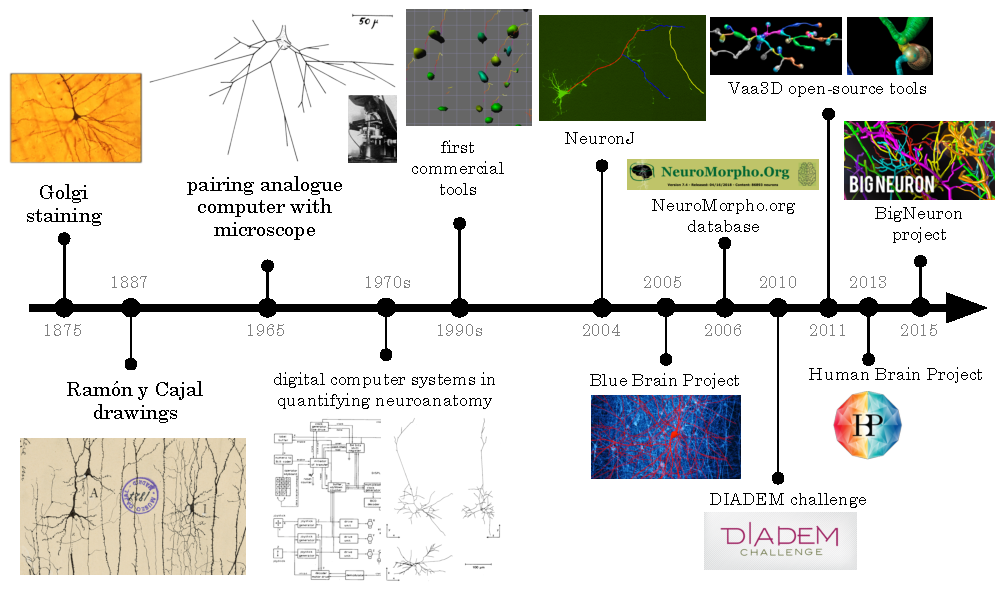
\includegraphics[width=\textwidth]{fig1}
	\end{center}
	\caption{Timeline overview of the selected accomplishments concerning to the neuron cell analysis. The impact of electrical engineering and computer science is crucial for the great achievements in recent decades.}
	\label{fig1}
\end{figure}

Neuron cell thus represents a core building block of the brain and the nervous system. It appears in variety of shapes (Figure~\ref{ch1_fig7}) and specializations \cite{ascolitrees}. The estimated number of neuron cells in a human brain amounts to striking 89 billion \cite{herculano2009human} - number comparable to the count of stars in the Milky Way galaxy. The dimension of each neuron can range from a few to several tens of micrometer with the neurite branch diameter typically measured in $\mu m$ scale. Each neuron is further connected to 50 thousand other neurons on average which results in an extremely powerful computational network and an very efficient information storage device. Intriguing mechanism of the brain functioning has recently emerged as an important research topic as the complex functionality of the brain defines much of the living organism activities, even the those abstract and subjective such as consciousness. Modeling the brain functionality is one of the grand unanswered questions of our era and central to diverse fields such as physics, mathematics, biology and recently prominent - computer science \cite{markram2015reconstruction}.

Neuron analysis gear has been adopting to the advancements of technical infrastructure available for the experimentation. Numerous technical obstacles have nevertheless persisted when reaching out to record the neuronal sample. This is primarily due to the physical and physiological difficulties and the generally intangible functioning mode of the nervous system. With the early analogue computers \cite{glaser1965semi}, it became possible to connect computer with microscope and automate tracing using analogue linear motion transducers as well as significantly speed up gathering of the information about the dendritic and axonal patterns. Subsequent generations of digital computers \cite{capowski1981accurate, capowski1977computer} brought further advances in the neuron reconstruction technique by introducing the computer graphics mixed with the neuron image and the advanced operator controls such as 3D joystick. The expansion of home PC hardware and software in late decades of the 20th century increased the impact of the informatics \cite{halavi2012digital}. Breakthrough of the conventional PCs made it feasible to throughput more computation and eventually implement in practice the algorithms that, although previously discovered, could not be directly implemented and shared between the users on a needed scale. It also marks the period when the first commercial and open-source academic software solutions emerge and grow (Fig.~\ref{fig2}) which to this day proved to be a steady trend. Reconstruction tool software is implemented in wide range of languages on different platforms and distributed over all regularly used operating systems \cite{meijering2010neuron, acciai2016automated}. The related work presented here focuses on Java implementation deployed within ImageJ \cite{abramoff2004image, longair2011simple, pool2008neuritetracer} and on c++ implementations for Vaa3D platform \cite{peng2014extensible}.

\begin{figure}[t!]
	\begin{center}
		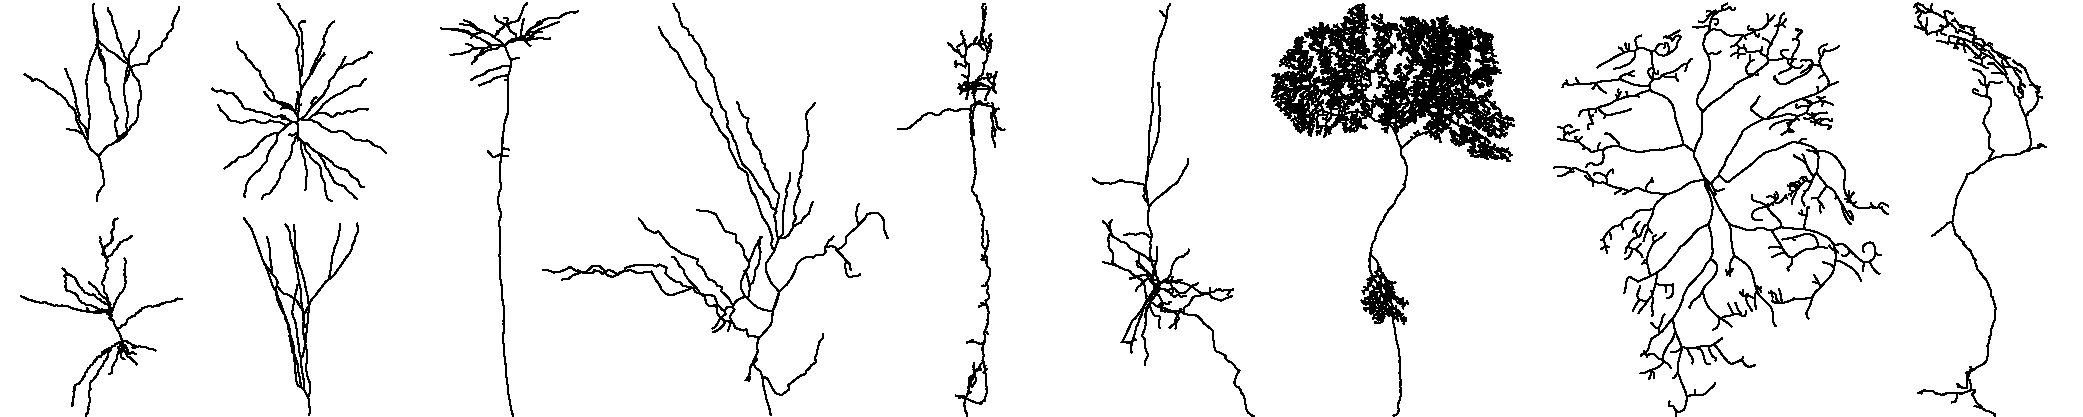
\includegraphics[width=\textwidth]{fig2}
	\end{center}
	\caption{Example neuronal branching arbors selected from the NeuroMorpho.org database. Showcase the topological diversity across multiple species, brain regions, and laboratories worldwide. Renderings exported using web-based neuron morphology viewer \cite{bakker2016web}.}
	\label{fig2}
\end{figure}

The crucial engineering tasks concerning the neuron reconstruction are: 1) need for the reduction of the time interval needed to compute the digital reconstruction and 2) most accurate possible reconstruction using often challenging data. The astonishing increase in the volume of acquired microscopy imaging data \cite{meijering2016imagining} undoubtedly raised the requirements bar when it comes to the time needed to for the reconstruction as images are increasingly larger and dedicated algorithms are needed to cope with the sized image volumes \cite{peng2017automatic}. Wide variety of neurons imaged under different modalities of the light microscopy (dark-field, bright-field, confocal) are still challenging for automated processing \cite{svoboda2011past, peng2011proof} and plethora of the reconstruction methods \cite{peng2011automatic} have ever since dealt with this task, resulting in two grand challenges such as DIADEM\footnote{http://diademchallenge.org} (``digital reconstruction of axonal and dendritic morphology'') and BigNeuron\footnote{http://bigneuron.org} \cite{peng2015diadem, peng2015bigneuron, gillette2011diademchallenge} (Fig.~\ref{fig1}) intended to stimulate the community effort and improve the overall state-of-the-art. In spite of the great advancements in the field, both tasks are yet very actual.

The physical appearance of the neuron cells takes part in the nervous system activity. Morphology of the single cell, shape of the neuronal network, topology or connectivity react to the external conditions or external stimuli. With the imaging tools such as fluorescence microscopy, the physical appearance the morphology of the single cell can be captured at micro meter scale can be inspected and recorded. In fact, the studies that require deeper analysis make use of the imaging techniques that reach nano meter scale, such as electron microscopy. In other words, accurate quantification of the cell shape is an important step towards better understanding of the cell functionality. Quantification of the neuronal structure is crucial in many neuroscience studies \cite{halavi2012digital} and quantification from microscopic images is identified as one of the major technical challenges in the digital era of neuroscience \cite{peng2015diadem}.

The advancements in informatics made it possible (Fig.~\ref{fig1}) to utilize computers to solve the neuroinformatics challenges over recent decades. With ever growing amount of data, processing of the gathered information still remains a challenge.   

\section{Capturing neuron morphology}
\label{sec:capturing-neuron}
Typically, imaging neurons consists of three main stages \cite{peng2015bigneuron}. First, the neuron sample is labeled in order to expose the structure, then the digital images are acquired using one of the microscopy modalities. Finally, the obtained neuron images are computer processed. In addition, the algorithms often require to be customized in order to address a particular biological question or be used in wider range of biological questions under wider range of image types which often prevents them from being used across different laboratories. The key obstacles in reaching the ubiquitous, accurate and robust automation of the neuron reconstruction \cite{meijering2010neuron, donohue2011automated, acciai2016automated} can be seen through the number of hampering factors which concern both the intricate nature of the data and the barriers imposed by the imaging modality. In this regard, it is possible to identify some major hurdling items.

\textit{Morphology} of the neuron cell is remarkably diverse (Fig.~\ref{fig2}). The structural intricacy of the complex examples can be challenging, even to the human visual comprehension. High complexity requires large amount of hours needed for manual delineation which thus inevitably becomes more error-prone. Hence the need for constant improvement of the computer vision algorithms. The aim of the methods is to reduce the manual labor time while fabricating trustful reconstructions. For instance, the 20-fold speedup of the reconstruction time compared to the manual reconstruction had been projected in earlier challenges \cite{liu2011diadem}.

\textit{Imaging} neurite arbor using different variations of light microscopy has been widely accepted choice for inspecting the cell structure \cite{meijering2010neuron, donohue2011automated}. Capturing $\mu$m scale objects (e.g. neurite diameter \cite{ascolitrees}), however, introduces imaging limitations. Optical systems suffer from the diffraction limit resulting in the single-lens imaged object point source being transmitted as the airy pattern \cite{cox2012optical}. In practice, the point source produces the point-spread function (\gls{psf}) which under reasonable assumptions can be approximated with the Gaussian \cite{zhang2007gaussian}. The lateral resolution in fluorescence microscopy is, nevertheless, such that the neurite dimensions are not substantially higher than the imaging resolution limits (sub-$\mu$m) which can be a limiting factor. Axial spatial resolution ($xy$ plane), on the other hand, is yet even (multiple times) lower as the precision is lost in the transition when imaging different stack layers ($z$ axis resolution). Eventually, the imaging process is predominantly affected by the particle-count driven photon noise \cite{van1998digital}, modeled with the Poisson process. Thus, the Poisson distribution is further used in generating synthetic microscopic images \cite{smal2010quantitative}. In accordance with the earlier studies, signal-to-noise ratio (\gls{snr}) of the microscopic image is expressed as the ratio of the intensity inside neuron above the background and the standard deviation of the noise inside neuron \cite{cheezum2001quantitative, smal2010quantitative}. Besides optical ``blurring'', neuron imaging can comprise pixelisation with the large spatial extent of the neuron. Combining together the optical magnification with the limited size of the digital matrix used to store the recording, as a consequence -the voxel size becomes larger that the \gls{psf} resulting in partial volume effect.% particles and debris can be erroneously detected as neuron structures

Burden of the ever increasing data volume size tends to counterbalance the increased memory and processing speed of commonly available modern computers. Although the automated tracing of the neuron morphology has substantially improved over the recent years, the existing methods do not scale well enough with the increased volume in terms of the processing speed and the accuracy. Typically, the methods are challenged if applied on datasets with very large neuronal image stacks \cite{peng2017automatic}. As a consequence, the image volume size represents a significant challenge for the computer vision methods. Dedicated strategies, such as extending the existing neuron tracing algorithms in order to be able to trace the unlimited data volumes \cite{peng2017automatic}, processing of the stitched imagery, or iteratively tracing in adjacent image tiles \cite{zhou2015neuron} have been reported.

\textit{Gold standard} of the neuron reconstruction is not an unique absolute digital representation of the image, but rather an (considerably subjective) approximation of the existing morphology. Often, the gold standard expert annotations are semi-automatic - thus obtained aided with various established tracing tools \cite{ascoli2007neuromorpho} both non-commercial such as NeuronJ \cite{meijering2004design}, open-source Vaa3D \cite{peng2014extensible} or the commercial packages such as Neurolucida (MBF Bioscience) or Amira (Thermo Fisher Scientific). With the often intricate structure of neuronal arbor, the expert annotations can differ and should be interpreted as a one among possible versions. Attempts to reach a consensus annotation by bringing together gold standards from different sources \cite{peng2015bigneuron}. Hence, the subsequent corrections (proof-editing) are often crucial in reaching better quality \cite{peng2011proof}. To attain optimal results in practice, additional expert corrections are often essential \cite{peng2011proof}. One way to overcome the obstacle is to use the consensus from several available gold-standard reconstructions as a better choice. Such scenario requires further definition on how the consensus would be computed. If the study concentrates on benchmarking the image analysis methods, synthetic neuron images can be generated from the existing reconstructions as the ground truth \cite{koene2009netmorph, radojevic2015fuzzy, radojevic-pnr}. This way, there is no need for multiple reconstruction sources as the real ground truth is known through reverse engineering.

Aforementioned items impose considerable barrier in attempt to consistently and efficiently produce digital reconstructions comparable with the expert ones.

\begin{figure}
	\centering
	\begin{tabular}{c@{\hspace{1em}}c@{\hspace{1em}}c@{\hspace{1em}}}
		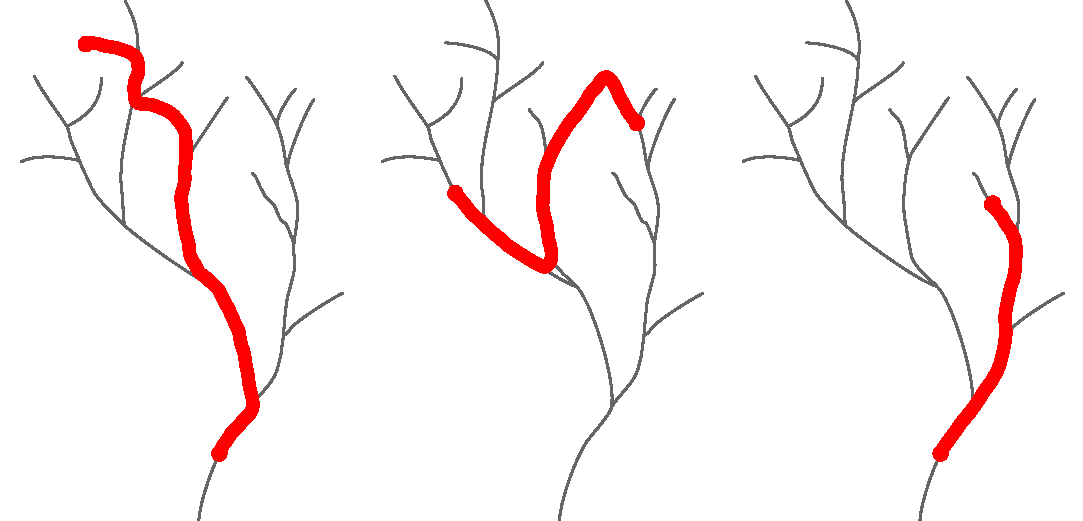
\includegraphics[width=0.3\textwidth]{fig3a} & 
		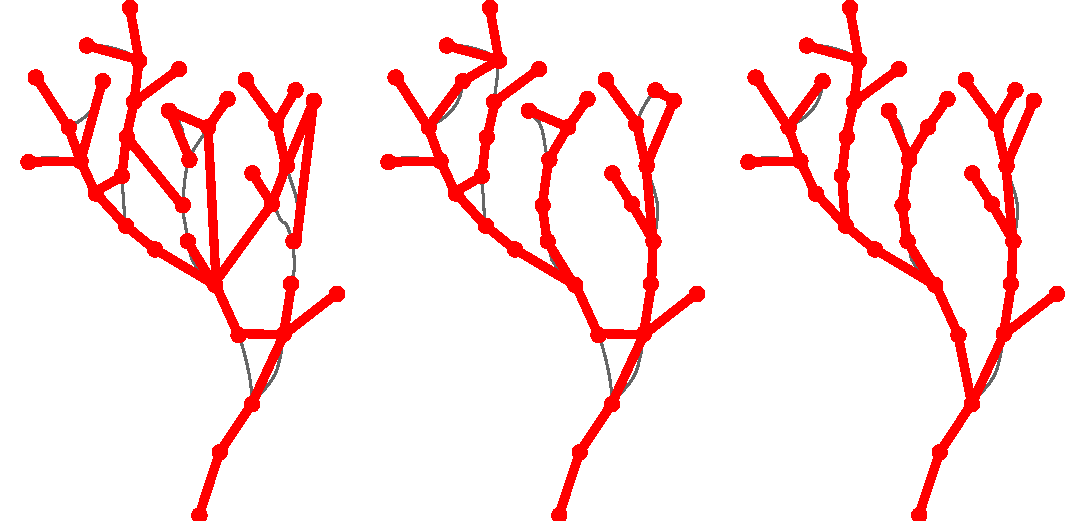
\includegraphics[width=0.3\textwidth]{fig3b} & 
		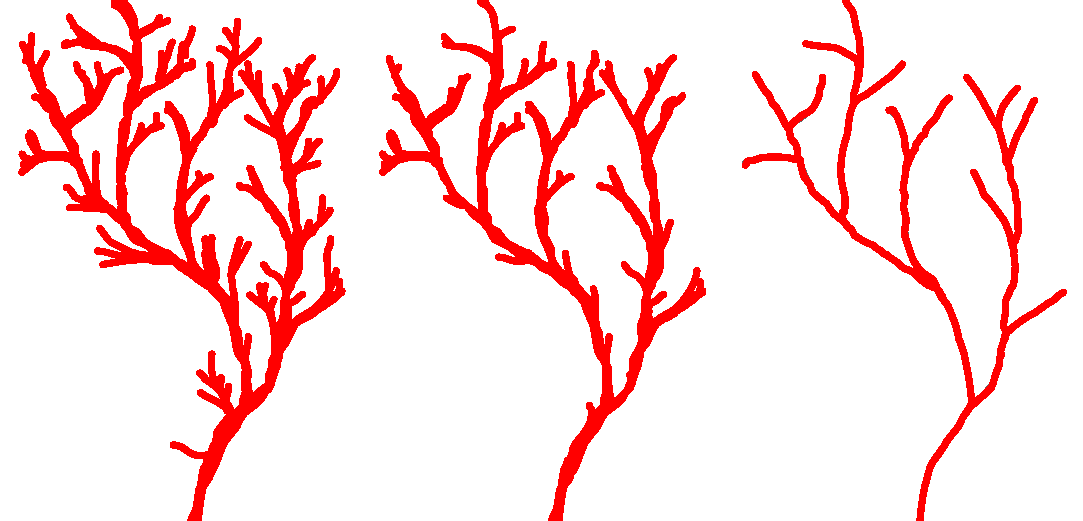
\includegraphics[width=0.3\textwidth]{fig3c} \\
		a) Shortest path tracing & b) Minimum spanning tree & c) Path-pruning
	\end{tabular}
	\caption{Examples of the essential neuron reconstruction strategies: a) Finding optimal path having two control points, b) Inferring the  optimal tree structure from the set of nodes c) Pruning the over-complete neuron tree.}
	\label{fig3}
\end{figure}

\section{Reconstructions from light microscopy}
\label{sec:reconstructions}
Strategies for neuron single cell reconstruction employ different algorithmic approaches. Vast majority of the introduced work treats tree reconstruction as loosely modular task where the pipeline of different algorithmic units are dedicated to handle processing of particular tree components \cite{meijering2010neuron}. Nevertheless, there is inevitably a degree of commonality and interdependence among the methodologies used, as the cascade of methods requires outputs used in one computation stages to be used in the follow up steps. The reconstruction accuracy also depends on the ability of the image analysis tool to generalize well which does involve undertaking a fair share of global reasoning. Extensive amount of the methodologies introduced over the years \cite{meijering2010neuron,donohue2011automated,acciai2016automated} can be broadly cast into three general approaches (strategies) (Fig.~\ref{fig3}) where each strategy emulates various optimization tasks: neurite tracing as an optimal path between given endpoints (Fig.~\ref{fig3}a), finding an optimal tree from the set of given landmark points that already belong to the tree (extracting the most accurate tree from the given set of guide points Fig.~\ref{fig3}b) and over-tracing/over-representing the tree (Fig.~\ref{fig3}c). As one might presume, the methodological separation cannot be absolute rigorous. It is very likely for the methods to combine together different ideas and overlap in terms of the approach used.

Neurite branch tracing can be interpreted as the energy/cost minimization problem \cite{meijering2004design,peng2010automatic} used to extract the trace or to refine the existing one. Classic example of neurite tracing is computing an optimal (shortest) path through the existing voxel grid where the designed geodesic metric or cost function has been defined to weigh the transition between grid elements (graph vertices). Such processing strategy has been particularly ubiquitous in practice \cite{meijering2004design,peng2010v3d,longair2011simple}, notably for semi-automated tasks where the control points of the optimized trace are initially known or had been computed. Notable tracing approaches are geodesic shortest path \cite{peng2010automatic} or live-wire segmentation \cite{meijering2004design} solved using Dijsktra shortest-path algorithm \cite{dijkstra1959note} - a methodology well established in tracing curvilinear structures. The downside of tracing defined in this manner is the necessity of having the control points - trace endpoints or correct initialization which can be challenging and require global image reasoning. Computed curve can further be refined with energy minimization and solved using gradient descent optimization \cite{peng2007straightening,peng2010automatic}. 

Given the output format used to store the digital reconstruction result (explained in more detail in Section~\ref{ch1_sec4}), digital neuron tree consists of the set of connected discrete neuron compartments (spherical nodes). Neuronal compartment would hence correspond to the cross-section of the branch segment. The essential geometrical quantities computed during tracing are the compartment 3D center $\mathrm{p} = (x, y, z)$ and the local (sphere) radius $r$ which would relate to the diameter of the segment. Depending on the tracing approach, neuron nodes can be also assigned with the direction $ \mathrm{v} = ( v_x, v_y, v_z ) $ computed at $\mathrm{p}$. The cumulative cost function used to steer the tracing toward an optimal solution is used within the optimization scheme and computed over the tract components. Aside from the geometrical constrains, also needs to include (take into account) the values extracted from the image - i.e. locally sampled/interpolated image intensity, or some other custom designed measure computed using (by filtering) local image intensities over the spatial extent of the node $\mathrm{x}$. For a more in-depth illustration, it is useful to introduce a vector $\mathrm{x} = \left[  \mathrm{p}, r, \mathrm{v} \right] $ combining all geometrical elements of the neuron compartment together. Sequence of digital neurite nodes $\mathrm{X} = \left\lbrace \mathrm{x}_1, ... , \mathrm{x}_i, ..., \mathrm{x}_N \right\rbrace$ would concatenate together the nodes that correspond to a digitized neurite tract (trace). Cumulative cost (Eq.~\ref{ch1_eq3}) computed over the tract would result in a measure whose minimization results with an optimal trace. Cost defined such way can be also used to define the energy being minimized to further refine the trace.

%\begin{equation}
%C(\mathrm{X}) = \int_{\mathrm{X}} c( \mathrm{x}, I(\mathrm{x}) ) d\mathrm{x}
%\end{equation}
%The trace segment with $L$ elements can be  $\mathrm{X}_L = \left\lbrace \mathrm{x}_i \right\rbrace, 1 \leq i \leq L $ containing $L$.

\begin{equation}
C(\mathrm{X}) = \sum\nolimits_{i} c(\mathrm{x}_i, I(\mathrm{x}_i)) \Delta\mathrm{x} 
\label{ch1_eq3}
\end{equation}

Cost function $ c( \mathrm{x}, I(\mathrm{x}) ) $ (Eq.~\ref{ch1_eq3}) typically represents a weighted score of the set of geometry and intensity based components. If expressed with two constituents for the illustration purpose, cost function would further decompose into:

\begin{equation}
c(\mathrm{x}, I(\mathrm{x})) = \alpha c_{\iota}(\mathrm{x}, I(\mathrm{x})) + (1-\alpha) c_{\gamma}(\mathrm{x}) 
\label{ch1_eq4}
\end{equation}

where $c_{\gamma}$ corresponds to the geometry-based and $c_{\iota}$ to an intensity-based component, with weight $ \alpha \in \left[ 0, 1 \right] $. 

The intensity-based component can directly use the sampled voxel intensities:
\begin{equation}
c_{\iota}( \mathrm{x}, I(\mathrm{x}) ) = I(\mathrm{x})
\end{equation}

where $I(\mathrm{x}) = I(\mathrm{p}) = I(x, y, z)$ represents the voxel intensity at given location. Alternatively, the exponential of the inverse intensity of pixels along the path can be used to define the cost \cite{peng2010automatic}:
\begin{equation}
c_{\iota}( \mathrm{x}, I(\mathrm{x}) ) = \text{exp} \left(  \lambda  (1 - \tilde{I}(\mathrm{x}))^2 \right)
\end{equation}

where $\tilde{I}(\mathrm{x})$ represents the normalized intensity value $ \tilde{I}(\mathrm{x}) = \tilde{I}(\mathrm{p}) = \tilde{I}(\mathrm{p}) / I_{\text{max}}$, with $I_{\text{max}} \equiv \max_{\substack{\forall \mathrm{p}}} \left\lbrace  I(\mathrm{p}) \right\rbrace $.

The custom tubularity measure $\rho$ can also be used to weight an intensity-based component:
\begin{equation}
c_{\iota}( \mathrm{x}, I(\mathrm{x}) ) = \rho(\mathrm{p}) = \rho(x, y, z)
\end{equation}

where $ \rho $ denotes the computed tubularity measure. If obtained over set of scales $\Sigma$, it becomes $\rho_{\Sigma}$ with $\Sigma = \left\lbrace \sigma_k \right\rbrace$, $1 \leq k \leq K$ used to denote the scales $\sigma$ used when filtering. Ratios of the Hessian eigen values obtained at different scales $\sigma_k$ are used to determine the scalar intensity which highlights the tubular structures \cite{sato19973d,meijering2004design,frangi1998multiscale}. Also the scale-space analysis of the line profile model \cite{steger1998unbiased} can be used. Thanks to the Hessian eigen-analysis, the tubularity (curvature) measure is computed \cite{sato19973d} which can also incorporate the local direction of the filtered tube-like structure \cite{frangi1998multiscale,meijering2004design}. Tubularity measures are commonly computed at pre-filtering stage and aim to reduce the presence of noisy, non-tubular structures. Tubularity measure calculated this way is deterministic and unsupervised  which implies usage of the predefined computation recipe regardless of the input data. Moreover, calculating the tubularity measure can also be cast as a supervised learning problem \cite{sironi2016multiscale,li2017deep} enabling tubularity measure to adopt to a particular problem based on the training. The practical downside of such approach, aside from designing the most suitable machine learning model, is that it requires dedicated training which in practice can be time and resource consuming.%closeness to local centers of image intensity distribution

Trace refinement can be based on the discrepancy of the node locations from the centers of the intensity distribution. Minimizing the energy computed as in Eq.~\ref{ch1_eq2} is used to further align the curve to the underlying image intensities.  
\begin{equation}
c_{\iota}(\mathrm{x}_i, I(\Theta(\mathrm{x}_i))) = \text{exp} \left( \lambda \frac{ \sum\nolimits_{\mathrm{y} \in \Theta(\mathrm{x}_i)} \lVert \mathrm{x} - \mathrm{y} \rVert^2 I(\mathrm{y}) \Delta\mathrm{y}  }{\sum\nolimits_{\mathrm{y} \in \Theta(\mathrm{x}_i)} I(\mathrm{y}) \Delta\mathrm{y} } \right) 
\label{ch1_eq2}
\end{equation}

$\Theta(\mathrm{x}_i)$ of the Eq.~\ref{ch1_eq2} denotes the local spatial neighborhood of the spherical node compartment $\mathrm{x}_i$. Such refinement scheme equates to the image intensity based mean-shift \cite{cheng1995mean} of the node location, which can also be used to refine a collection of the overlapping tracings \cite{radojevic-pnr}.

Zero-mean normalized cross-correlation (\gls{zncc}) is a normalized, contrast-independent measure used to quantify the similarity of the encountered intensities sampled within the node compartment with the given spatial intensity distribution model.
\begin{equation}
c_{\gamma}(\mathrm{x}_i, \Phi(\mathrm{x}_i)) = \frac{ \sum\limits_{\mathrm{p} \in \Phi(\mathrm{x}_i)} (I(\mathrm{p}) - \bar{I}(\mathrm{p}))(G_{\sigma}(\mathrm{p}) - \bar{G}_{\sigma}) }{ \sqrt{ \sum\limits_{\mathrm{p} \in \Phi(\mathrm{x}_i)}(I(\mathrm{p}) - \bar{I}(\mathrm{p}))^2 \sum\limits_{\mathrm{p} \in \Phi(\mathrm{x}_i)}(G_{\sigma}(\mathrm{p}) - \bar{G}_{\sigma})^2 } }
\label{ch1_eq1}
\end{equation}

$\Phi(\mathrm{x}_i)$ represents the spatial neighborhood of the node compartment $\mathrm{x}_i = [ \mathrm{p}, \mathrm{v}, \sigma ]$, commonly defined as the tube cross-section cylinder centered at $\mathrm{p}$, having $\sigma$ radius and directed along $\mathrm{v}$. $\bar{I}$ and $\bar{G}$ are the respective mean values of the intensities inside the sampled region $\Phi$. $G_{\sigma}$ denotes the spatial intensity distribution model at given scale (cylinder radius) $\sigma$. In case of neurons - a Gaussian intensity profiles in the cylinder cross-section plane are a reasonable choice \cite{radojevic2017neuron}. 

The geometry-based component can incorporate the vectorial (directional) alignment of the centroids along the filtered tubularity direction \cite{meijering2004design}:  
\begin{equation}
c_{\gamma}(\mathrm{x}) = c_{\gamma}(\mathrm{x}_{i}, \mathrm{x}_{i+1}) = 1/2 \left( \varphi(\mathrm{p}_i, \mathrm{p}_{i+1})^{\frac{1}{2}} + \varphi(\mathrm{p}_{i+1}, \mathrm{p}_{i})^{\frac{1}{2}} \right) 
\end{equation}
where $\varphi( \mathrm{p}_{i}, \mathrm{p}_{j} ) = | \mathrm{v}_i \cdot \mathrm{u}_{ij} |  $ quantifies the alignment of the curve - amount of the directional overlap of the local tubularity direction with the unit link vector between the two points $\mathrm{u}_{ij} = (\mathrm{p}_j - \mathrm{p}_i) / \lVert \mathrm{p}_j - \mathrm{p}_i \rVert $. Furthermore, the geometry-based measure such as the digital trace smoothness \cite{peng2010automatic} or bending energy \cite{radojevic2015fuzzy} is derived using the topological information:
\begin{equation}
c_{\gamma}(\mathrm{x}) = c_{\gamma}(\mathrm{x}_{i-1}, \mathrm{x}_{i}, \mathrm{x}_{i+1}) = \sum\nolimits_{i} (- \mathrm{p}_{i-1} + 2\mathrm{p}_i - \mathrm{p}_{i+1})^2 \Delta\mathrm{p}
\end{equation}

Besides Dijkstra shortest path tracing, numerous other versions of optimized local tracing have been reported. Energy-minimization techniques such as active contours had been adopted to determining the optimal parametrized skeleton \cite{schmitt2004new}, or directly to the open-curve contour using gradient-vector flow to optimize the energy \cite{wang2011broadly}. Although the path optimization methods do require the initialization in form of control points as a crucial step, the active contours would further refine the initialization allowing starting points to align better according to the local image context. The general downside of such approach, however, is the possibility of forming the gaps due to the discontinued neurite segments in low quality images. 

Fast marching (FM) algorithm \cite{sethian1999level} have been reported of being used in neuron reconstruction \cite{xiao2013app2,  peng2011automatic, mukherjee2012automated, van2007subvoxel, santamaria2015automatic, basu2014reconstructing}. Conceptually similar to Dijkstra shortest path, FM turned out to be particularly useful in delineating the curvilinear structures and also due to the ability to bridge the gaps between the disconnected neurite segments. FM solution as a fast numerical solution to the Eikonal equation, in essence very similar to Dijkstra algorithm, has been used to gradually grow the segmented neuron region by connecting the neighboring neurite segments with the growing body \cite{peng2011automatic}. Particular implementations of FM-based reconstruction (i.e. APP2 method \cite{xiao2013app2}) have been very effective in reducing the existing false-positives in preceding approaches \cite{van2007subvoxel, peng2011automatic}. Follow-up FM contributions report the improvements related to speed tracing of the discontinuous segments, principally with the usage of the gradient descent combined with the re-initialization \cite{mukherjee2012automated} and the back-tracking \cite{liu2016rivulet} to overcome the challenging interrupted structures.  

%-------------------------------------------------------
Accurately merging the obtained tracts or the control points into a tree reconstruction (Fig.~\ref{fig3}b,c) represents a significant challenge. Due to the complexity of the problem (many alternatives to explore and evaluate) and the amount of computation needed to exhaust the search in order to reach the optimal solution, assembling a correct neuron tree structure is often solved through an approximation while correctly combining together the shared portions of the branch remains an ongoing challenge \cite{peng2015bigneuron}.

Significant share of the methods aims at finding a globally optimal solution. The set of node candidates is then commonly turned into a weighted graph with the reconstruction based on extracting the optimal tree out of the weighted graph. Prominent method for this purpose is the NP\footnote{non-deterministic polynomial-time}-complete minimum spanning tree (\gls{mst}) algorithm \cite{turetken2011automated, yuan2009mdl, gonzalez2010delineating, xie2010automatic}. Often used solution is to extract minimum trees spanning subset of the graph edges - however, the solution to such problem is a complex NP-hard \cite{chimani2009obtaining} involving plenty of exploration scenarios, and the approximative solutions are used in practice \cite{blum2005combining, gonzalez2010delineating}.

MST typically involves the detection of generally referred to as - control points (also named the anchor-, saddle-, seed- or critical points in various sources) where MST algorithm is subsequently used for merging the obtained points into a tree in an optimal manner. Control points are location where selected measure reaches a stationary point. It can be curvature computed from the Hessian eigen-analysis \cite{yuan2009mdl}, or the set of anchor points computed using supervised learning \cite{turetken2011automated}. Substantial number of solutions \cite{gonzalez2010delineating, xie2010automatic, turetken2011automated} base the dendritic arbor reconstruction on finding a K-Minimum Spanning Tree (k-MST) which spans subset of K control points optimizing a global objective function using approximate solutions of the original MST spanning all control points. The MST is used to link the control points establishes connections using various criteria for linking and weighting different structures. Therefore, the optimization can be based on the image intensities and the distance \cite{yuan2009mdl}, or the probabilistic costs computed based on the proximity of path elements towards the middle of a filament \cite{turetken2011automated}.

Finally, particularly protruding family of methods that employ the pruning strategy (Fig.~\ref{fig3}c) is used to reconstruct the neurons. Such methods start with the over-reconstruct neuron tree and gradually reduce (``prune'') the reconstruction converging towards the optimal concise sub-tree neuron representation. The underlying idea is to capture all pixels belonging to a neuron in a graph and subsequently iteratively discard particular graph components using an optimized pruning procedure. In all-path pruning (\gls{app}) \cite{peng2011automatic}, traces are obtained using Dijkstra shortest path, while the iterative pruning starts with the leaf nodes of the over-reconstruction. It executes in linear time, ensuring the maximum coverage and minimum redundancy of the underlying neuron signal. The graph nodes that are already covered by others are removed with higher priority. Similar principle is applied in the follow-up work \gls{app2} \cite{xiao2013app2} where several improvements have been introduced - namely the APP2 employs a long-segment-first hierarchical pruning and uses the dedicated preprocessing of the input image stack intended to optimize the fast-marching based tracing. 

The downright number of published computational recipes is in sharp contrast with the fact that manual or semi-automated delineation is among the very common tools used by the neurobiologists. Along with the actual practical robustness and relatively modest versatility of the implemented tools, it indicates that the monolithic computer vision solution for the neuron arbor reconstruction is yet to be unraveled. The existing toolbox consists of number of archetypal approaches, incorporated through the large amount of variations and incremental improvements. Whether it is the usage of the overcomplicated geometrical assumptions, or the inability to take into account all the complexity encountered with neuron - reconstruction methods have not been able to achieve perfect robustness and stay in demand for the original approaches. The practice suggests that the accurate and robust neuron reconstruction depends on the right balance between global and local processing. Correct generalization still remains a challenge and is essential for the algorithm success. 

\subsection{Bayesian filtering in neuron tracing}
Bayesian reasoning operates with the assumption that the computed quantities are not measurable directly but possible to estimate (filter) within two essential processing stage cycles: prediction and update \cite{doucet2001introduction}. As a result, the posterior distribution, outcome of the full cycle of two prediction-update filtering stages can be iteratively computed leading to a recursive estimation. Tracing neurite branch cross-section is also a variant of spatial filtering: the position of current and follow-up neurite node compartment can be iteratively filtered with the aforementioned recursion. Thus, estimating the unknown (hidden) quantities, included in hidden state vectors $ \left\lbrace \mathrm{x}_t, t \in \mathbb{N},  t \geq 0 \right\rbrace $ using sequentially arriving observations $ \left\lbrace \mathrm{z}_t; t \in \mathbb{N}, t > 0 \right\rbrace $ leads to the joint posterior distribution of the defined state vector values. Quantification of the neuron compartment values stored in $\mathrm{x}$ - neurite tracing - is hence the estimation of their probability density further defined as computation of the posterior for given hidden states. The value $\hat{\mathrm{x}}$ computed from the posterior distribution $p(\mathrm{x})$ (e.g. weighted average) serves as a final filtering outcome.

In such constellation, tracing is defined as a recursive utilization of the Bayes' theorem (Bayesian filtering) which yields sequential computation of the hidden state-vector posterior distribution using the conditionally independent measurement directly acquired from the image $ p(\mathrm{x}_t |  \left\lbrace  \mathrm{z}_1, \mathrm{z}_2, ..., \mathrm{z}_t \right\rbrace  ) $.

The estimation operates recursively, continuously predicting and updating the joint distribution of the hidden states \cite{doucet2001introduction}. The recursion mechanism hence uses the modeled prior transition $ p(\mathrm{x}_t | \mathrm{x}_{t-1}) $ as a basis for the motion model and to predict the hidden state prior distribution using the already available knowledge. The likelihood $ p(\mathrm{z}_t | \mathrm{x}_t) $ used to update the predicted quantities relates them to the continuously arriving observations. In case of spatial filtering, the motion model is embedded within the prediction mechanism.

The joint posterior distribution of the vectors that have been estimated up until time $t$, denoted with $\mathrm{x}_{0:t} \equiv \left\lbrace \mathrm{x}_1, \mathrm{x}_2, ... \mathrm{x}_t \right\rbrace  $ contains the trace quantities - for instance - the neuron compartment values introduced earlier in this section. Joint posterior distribution is therefore estimated using the observations $\mathrm{z}_{1:t} \equiv \left\lbrace \mathrm{z}_1, \mathrm{z}_2, ... \mathrm{z}_t \right\rbrace $ sequentially gathered up until the time $t$. The joint posterior $ p(\mathrm{x}_{0:t} | \mathrm{z}_{1:t}) $ is determined using the Bayes' theorem \cite{doucet2001introduction,ristic2004beyond} and computed recursively, with each iteration $t$, being derived knowing the posterior of previous iteration.
\begin{equation}
p(\mathrm{x}_{0:t} | \mathrm{z}_{1:t}) = \frac{p(\mathrm{z}_{1:t} | \mathrm{x}_{0:t}) p(\mathrm{x}_{0:t})}{\int p(\mathrm{z}_{1:t} | \mathrm{x}_{0:t}) p(\mathrm{x}_{0:t}) d\mathrm{x}_{0:t} }
\label{ch1_eq5}
\end{equation}
 
The marginal distribution $ p(\mathrm{x}_t | \mathrm{z}_{1:t}) $ is computed by reiterating the prediction (Eq.~\ref{ch1_eq6}) - update (Eq.~\ref{ch1_eq7}) sequence:
\begin{equation}
p(\mathrm{x}_t | \mathrm{z}_{1:t-1}) = \int p(\mathrm{x}_t | \mathrm{x}_{t-1}) p(\mathrm{x}_{t-1} | \mathrm{z}_{1:t-1}) d\mathrm{x}_{t-1}
\label{ch1_eq6}
\end{equation}

\begin{equation}
p(\mathrm{x}_t | \mathrm{z}_{1:t}) = \frac{p(\mathrm{z}_t | \mathrm{x}_t) p(\mathrm{x}_t | \mathrm{z}_{1:t-1})}{ \int p(\mathrm{z}_t | \mathrm{x}_t) p(\mathrm{x}_t | \mathrm{z}_{1:t-1}) d\mathrm{x}_t}
\label{ch1_eq7}
\end{equation} 

Following from Eq.~\ref{ch1_eq6} and ~\ref{ch1_eq7}, posterior probability distribution of the state $\mathrm{x}_t$ knowing measurements $\mathrm{z}_{1:t}$ is defined with the recursion:  
\begin{equation}
p(\mathrm{x}_t | \mathrm{z}_{1:t}) \propto p(\mathrm{z}_t | \mathrm{x}_t) \int p(\mathrm{x}_t | \mathrm{x}_{t-1}) p(\mathrm{x}_{t-1} | \mathrm{z}_{1:t-1}) d\mathrm{x}_{t-1}
\label{ch1_eq8}
\end{equation}
where current probability distribution is computed recursively, driven by the prior-modeled prediction $p(\mathrm{x}_t | \mathrm{x}_{t-1})$ and update based on the computed likelihood $p(\mathrm{z}_t | \mathrm{x}_t)$. The layout of Bayesian filtering framework allow custom design of any of the algorithm components, making it a fairly universal tool that resulted in many solutions \cite{sarkka2013bayesian}.    

Several well-known analytical solutions to Bayesian filtering, such as the prominent Kalman filter (KF) or Hidden Markov Model filter are based on mathematical assumptions that turn out to be limiting factor in practice. For instance, the closed-form solution in case of Kalman filter is constrained  with the linear-Gaussian signal-observation model assumptions imposed on the state model. Numerous other approximation schemes (extended KF, grid-based filters) have been proposed over the decades with varying accuracy, practical feasibility and computation cost. 

\begin{equation}
\left\lbrace \mathrm{x}_{0:t}^{(i)}; i = 1, ... , N \right\rbrace 
\label{ch1_eq9}
\end{equation}

Sequential Monte Carlo (\gls{smc}) approximation methods \cite{arulampalam2002tutorial} on the other hand do not adhere to the aforementioned limitations, but instead offer an approximate simulation-based approach where a number of random samples \footnote{The term particles can be used interchangeably within SMC related content of this thesis.} (Eq~\ref{ch1_eq9}) according to $p(\mathrm{x}_{0:t} | \mathrm{z}_{1:t})$ approximates the filtered posterior distribution so that the intractable integration of the Eq~\ref{ch1_eq7} and ~\ref{ch1_eq8} is approximated with number of samples drawn - more samples leading to a better approximation offering a common generic solution for tasks involving non-Gaussian, non-linear state-space model or high dimensionality. SMC method can be generalized for variety of problems, it is applicable to a wide set of models, straightforward to implement and used in different contexts. Such qualities are particularly convenient as it leaves plenty of possibilities for customization of the algorithm stages. Moreover, the filtering can be used as an independent component of the larger algorithm. 

\begin{equation}
\tilde{w}_{t}^{(i)} \propto \tilde{w}_{t-1}^{(i)} \frac{p(\mathrm{z}_t | \mathrm{x}_{t}^{(i)}) p(\mathrm{x}_{t}^{(i)} | \mathrm{x}_{t-1}^{(i)} )}{ \pi(\mathrm{x}_{t}^{(i)} | \mathrm{x}_{0:t-1}^{(i)}, \mathrm{y}_{1:t}) }
\label{ch1_eq10}
\end{equation}

\begin{equation}
\tilde{w}_{t}^{(i)} \propto \tilde{w}_{t-1}^{(i)} p(\mathrm{z}_t | \mathrm{x}_{t}^{(i)})
\label{ch1_eq11}
\end{equation}

The classical SMC filtering solution assigned the importance weight $w^{(i)}(\mathrm{x}_{0:t})$ to each sample based on the importance sampling (IS) distribution. However, such methods were not able to perform recursive estimation efficiently and the computational complexity due to the growing state sequence increased with time. This obstacle was overcome with sequential importance sampling (SIS) that allowed the importance function $\pi(\mathrm{x}_{0:t} | \mathrm{z}_{1:t})$ at time $t$ to be expressed as a function of the importance function at $t-1$ leading to the recursive computation of the importance weights $w_{t}^{(i)}$ (Eq~\ref{ch1_eq10}).

The weight deterioration over time in case of SIS method leads to the severe particle degeneration and a very sparse particle distribution. As a consequence, approximation fails to represent given posterior adequately. The breakthrough in adopting the SMC filtering methods to practical applications came along with the introduction of the bootstrap filter \cite{gordon1993novel}. The idea of resampling existing distribution particles so that those having higher importance weights are multiplied more - yielding their offspring becoming more numerous and equalizatio of the weight distribution upon the resampling.

Although the very first practical implementations were hampered by the computation requirements, modern computers can nowadays comfortably handle the algorithms. SMC methods are also presented as Particle Filters (\gls{pf}) and the two terms can be used interchangeably. In Chapter~\ref{ch4:pnr} of this thesis, a method for automated neuron reconstruction based on the Particle filter is proposed. Furthermore, the SMC method was also used in Chapter~\ref{ch3:phd} to solve of the multi-object Bayesian filtering also aimed at reconstructing the neuronal arbor. 

% https://www.neuron.yale.edu/phpBB/viewtopic.php?t=3477
% http://www.neuromorpho.org/myfaq.jsp (What is SWC format?)
% http://research.mssm.edu/cnic/swc.html
% http://www.neuronland.org/NLMorphologyConverter/MorphologyFormats/SWC/Spec.html
\section{Neuronal reconstruction format}
\label{sec:format}
Once processed, neurons are typically exported into a dedicated data format intended to store the idiosyncratic tree-like topology of the cell. Among different ideas and implementations of standards used for storing reconstructed neurons, two neuron morphology file formats prevail in lab usage and recent large scale neuron related projects \cite{bakker2016web}: Neurolucida DAT format (MicroBrightField, Inc.) and \gls{swc} format \cite{cannon1998line}. Neurolucida DAT format is closed-source binary format whose reverse engineered description\footnote{http://neuronland.org} suggests neuron compartments being saved as a hierarchical tree of the linear segments. SWC format on the other hand is open-source, space delimited text format that stores tree structure in an array $\mathcal{N} = \{ n_1, \dots , n_i, \dots , n_j, \dots  \}$ where each element of the array, $n_i$, corresponds to a neuronal spherical compartment (Fig.~\ref{fig4}d). SWC, therefore, renders the reconstruction as a list of nodes (neuronal compartments) with seven attributes: node index identifier $i$, node type, sphere 3D coordinates $(x_i,y_i,z_i)$, radius $r_i$ and a parent node index (Fig~\ref{ch1_fig5}). Parent node index represents the link towards predecessor node. By convention it is set to -1 for the origin node. To conform with a tree structure, each spherical compartment may have one predecessor (parent) with lower node index ($i<j$, Fig.~\ref{fig4}). Loops and disconnected branches should not exist as that would not be in agreement with the tree-like structure. Etymologically, SWC represents the acronym containing the initials of the last names of Stockley, Wheal, and Cole. Although not directly described in their joint work on quantitative measurement and modeling of the neuron morphology \cite{stockley1993system}, the origin of the SWC name is an acronym of the initials of their last names. 

Lastly, the SWC format exhibits variations, especially concerning the unified definition of the soma reconstruction \cite{bakker2016web}. Several interpretation of the standard exist\footnote{http://research.mssm.edu/cnic/swc.html}\footnote{http://www.neuronland.org/NLMorphologyConverter/MorphologyFormats/SWC/Spec.html}\footnote{NeuroMorpho.org FAQ: What is SWC format? http://www.neuromorpho.org/myfaq.jsp}. One of the downsides of the SWC format is its often oversimplified cylinder model of the soma. Being a rather simple (straightforward to implement the software to read and export) and open-source format, easy for exchange - it has been adopted by notable large-scale neuron morphology projects \cite{ascoli2007neuromorpho,peng2015bigneuron}. Some reconstruction methods even base the reconstruction methods on the SWC format \cite{feng2015neutube}. The work showcased in this thesis will exclusively use open source SWC format.
 
\begin{figure}
\begin{center}
	\begin{tabular}{c@{\hspace{0.75em}}c@{\hspace{0.75em}}c@{\hspace{0.75em}}c@{\hspace{0.75em}}}
	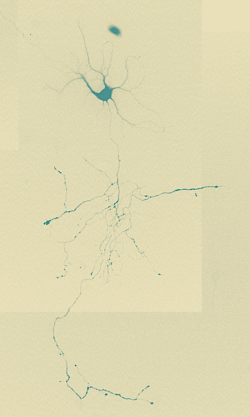
\includegraphics[align=c,width=0.2\textwidth]{fig4a} & 
	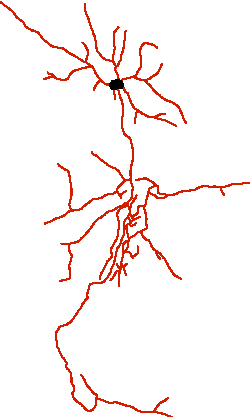
\includegraphics[align=c,width=0.2\textwidth]{fig4b} & 
	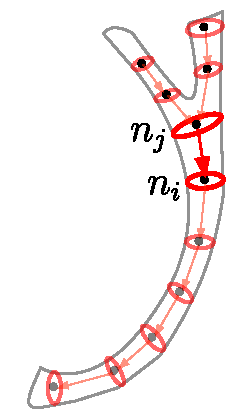
\includegraphics[align=c,width=0.2\textwidth]{fig4c} &
	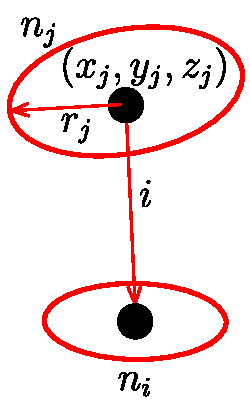
\includegraphics[align=c,width=0.2\textwidth]{fig4d} \\ 
	a) & b) & c) & d)
\end{tabular}
\end{center}
	\caption{Neuron morphology digital format data structure: a) Single neuron image, b) Digital reconstruction of the given neuron c) Illustration of the SWC format \cite{cannon1998line} used to store the digital reconstruction idiosyncratic tree structure $\mathcal{N} = \{ n_1, ... , n_i,..., n_j, ... \}$, d) Detailed visualization of the linear segment (truncated cone) connected pair of neuron compartments $(n_j, n_i)$ along with the component elements. Reconstruction exported using web-based neuron morphology viewer \cite{bakker2016web}.}
	\label{fig4}
\end{figure}

% does not need to be based on the distances or the overlap
Scientific evaluation typically requires computed neuron reconstruction to be evaluated. The evaluation is commonly carried out by comparing the obtained reconstruction (node tree) against the agreed gold standard - i.e. the most accurate reference representation available. In this regard, measuring the reconstruction quality boils down to quantifying resemblance between two neuron reconstructions (node tree pair). The comparison is traditionally based on the Euclidean distance -- inter-node spatial distances computed at each node measuring the metric distance towards corresponding closest node from the other tree. Besides, comparison can be based on the inter-node overlap resulting in retrieval measures like precision and recall. Furthermore, the comparison could be based on other quantitative measures computed from the given reconstruction that could also serve as a comparison footprint. Tools such as L-measure \cite{scorcioni2008measure} and Neuro-blast \cite{wan2015blastneuron} provide with the implementation for computing tree-feature quantities.  

\section{Thesis outline}
\label{sec:outline}
This thesis primarily addresses the need for further automation of the methods for neuronal image analysis. The thesis showcases the methodological contributions and experimental results obtained while investigating computer vision problems applied on microscopy images of neuron cells. Several original bioimage analysis computer vision approaches have been outlined throughout each chapter. Fundamental quantitative neurobiology problems such as digital reconstruction and tracing of the 3D image stacks containing single-neuron, detection of regions comprising neuronal morphology, and the localization of tree landmarks such as junctions and terminations (\textit{critical points}) have been investigated in separate sections. Each research topic is bundled with the methodological study, software implementation and had been experimentally evaluated. This thesis presents the obtained results of the research study.

Detecting critical points of the tree structure, among many other vision-related tasks, is in practice too complex to be modeled with a concise strict detector that is based on the plain intensity/shape comparison. However, it sounds faithful to loosely define the junction as a point where three streamlines of certain configuration pattern merge together. Similarly, the terminal point would correspond with the one where only one streamline segment can be distinguished in the local neighborhood. In Chapter~\ref{ch2:fuzzy}, critical point detector based on the fuzzy logic and rule-based reasoning had been introduced. The problem was approached as a fully automatic, unsupervised, localization and characterization of both types of aforementioned critical points in fluorescence microscopy images of neurons. The essential features about the main streamlines are obtained using directional filtering and stored using (fuzzified) linguistic terms. A custom-tailored set of dedicated rules structured as an IF-THEN questionnaire is then accumulated and evaluated over the set of features (linguistic terms) leading to a joint decision used to indicate the singularity points. The very concept of fuzzy set allows engineering partial membership towards the defined linguistic terms and thus helps modeling the uncertainty, especially convenient when trying to find the soft boundary between the categories. The ability to define the collection of general rules that can be truthful \textit{to a degree} is a convenient tool for fusing the information together into an aggregated decision. 

Central subject of the thesis is the utilisation of probabilistic methodology to resolve the image analysis problems related to the reconstruction of challenging neuron cell imagery. Non-deterministic Bayesian filtering approach has been a main framework of choice used to undertake two very important tasks: tracing (Chapter~\ref{ch3:phd}) and reconstruction (Chapter~\ref{ch4:pnr}) of the idiosyncratic tree-shaped structures in 3D microscopy stacks. In this regard, versatile Sequential Monte Carlo (\gls{smc}) method toolbox had been adopted to address the respective tasks. Following the Bayesian paradigm, the intent is to blend the prior model with the image measurements in two different fashions: single-object and multi-object tracking framework. Neurite tracing is therefore cast as an object filtering problem where the object of interest is a neurite cross-section. 

In Chapter~\ref{ch3:phd}, proposed multi-object filtering framework based on the probability hypothesis density (PHD) filter \gls{phd} represents a way to formalize the concept of simultaneous tracing of multiple neurites within the neuron arbor. Joint trace approach extends the existing probabilistic tracking to the next generalization level. This represents a step forward in perceiving the trace function, as reconstruction algorithms continue to evolve and mature. The PHD filter was implemented using dedicated \gls{smc} estimation \cite{ristic2010improved} reporting the results comparable to the state-of-the-art showcased in \cite{radojevic2017automated}.

The neuron reconstruction approach based on probabilistic tracing is described in Chapter~\ref{ch4:pnr}. Introduced strategy - named probabilistic neuron tracer (PNR) - is based on repeated, non-deterministic (over-)tracing of the neuron arbor. Set of probabilistically independent tracings is triggered using single object filtering followed by the trace refinement and grouping. Tracings are instantiated from the collection of seed neuron segments positioned along the high tubularity regions. Such technique enables additional repeated tracing, where the same arbor is re-examined with different initial conditions, and traced again based on a new, independent trace history. The inherit randomness eventually results with multiple reconstructions and gives higher importance to the more densely outlined segments that have been traced statistically more often. This strategy is helpful in case of structural ambiguities which tend to be frequently appearing with neuronal imagery. The PNR method represents a substantially redesigned work inspired with the entry method for the BigNeuron challenge \cite{peng2015bigneuron}.

Finally, in Chapter~\ref{ch5:ndetchml}, a feasibility study is presented. Supervised machine learning was used to discriminate the rectangular regions which contain single-neuron morphology. This task is conceived as a part of the high-throughput analysis pipeline where those regions containing neuron are extracted out from the background using machine learning as differentiation tool. The neuron patches are therefore discriminated against the background and detected within a large 2D high-throughput screening mosaic containing the neuron culture consisted of the scattered individual neurons. The classification is based on more-traditional visual features (e.g. \gls{sift} \cite{lowe2004distinctive}) combined with the assembly of texture, energy and transform \cite{orlov2008wnd} compared performance against several state-of-the-art classifiers to assess the limitations and feasibility using the more traditional tooling.

% outlined work provides with the implementation of multi-object based neurite tracking
% accurate till certain degree
% indicate the presence of the modeled cross section
% provides the frame to the likelihood measurement
% showcased methods that cope with uncertainty
% neuron processing offers a practical solution for the whole-
% quantifying the node presence by weighing the similarity against Gaussian-profiled cylinder model
% offers a possibility
Several contributions are highlighted. The experimental results of Chapter~\ref{ch3:phd} and Chapter~\ref{ch4:pnr} indicate that different forms of Bayesian filtering can be successfully applied (adjusted) to neuron reconstruction task and provide with state-of-the art precise traces using introduced prediction and update model. Proposed multi-object tracking represents a further generalization step in bridging together some of the earlier existing frameworks, which outlines a potential strategy for parallelized and context-aware reconstruction. Non-deterministic tree digitization is based on the assumption that there are multiple tracing alternatives to the same structure and that their aggregation yields the final solution. Also, the relevance of model-based reasoning is revisited: Gaussian intensity profile \cite{zhao2011automated, radojevic2017neuron} of the cross-section (in accordance with the \gls{psf} approximation) is used to model the smallest building block of the neuronal tree - neuron cross-section segment. Zero-mean normalized cross-correlation (\gls{zncc}) of the intensity values within the designated segment substitutes thresholding absolute measure derived from the intensity but instead uses the contrast-independent similarity as a localization gauge. Experimental evaluation in Chapter~\ref{ch3:phd} and Chapter~\ref{ch4:pnr} include synthetic neuron images generated from existing ground truth over different levels of \gls{snr}. Analyzing such imagery provides with a technical foundation aimed at benchmarking the method against varying levels of noise. Furthermore, a fairly objective comparison in neuron imagery can be carried out as the accuracy of the gold standard reconstruction in practice is often ambiguous or even subjective.